\documentclass[usenames,dvipsnames,tikz]{standalone}
\usetikzlibrary{patterns}
%\usepackage{amsmath,amssymb}
%\usepackage{xcolor}
\colorlet{tBlue}{RoyalBlue!35!Cerulean}
\colorlet{tRed}{Red}
\definecolor{tLightPink}{HTML}{FFD4EB} %tikz color
\definecolor{tLightOrange}{HTML}{FFE3B2}
\definecolor{tLightYellow}{HTML}{FFFBBD} %tikz color
\definecolor{tLightGreen}{HTML}{D3ECAA}
\definecolor{tDarkGreen}{HTML}{9BBF86} %tikz color %9BBF86
\definecolor{tTurquoise}{HTML}{ACFFEF} %tikz color %6FC4DD %7FE8F3
\definecolor{tLightBlue}{HTML}{CEF0FF} %tikz color %CEF0FF
\definecolor{tDarkBlue}{HTML}{95B5FF} %tikz color %95B5FF
\definecolor{tLightPurple}{HTML}{D8CFFD} %tikz color %ECDBFF
\definecolor{tPeach}{HTML}{F98F96} %tikz color %F98F96
\begin{document}
	
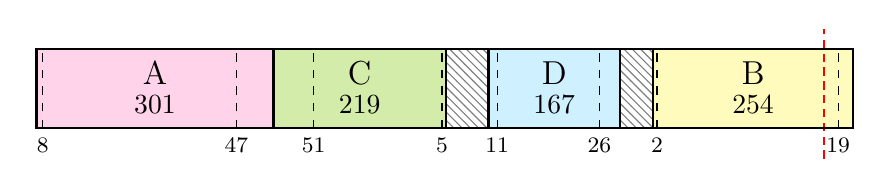
\begin{tikzpicture}
%\draw [help lines] (-1,-2) grid (11,5);
% 1=0.1, 2=0.15, 3=0.2, 4=0.25, 5=0.3
% 6 (3-27), 5 (8-42), 4 (33-65), 4 (16-22), 3 (13-28), 3 (11-40), 2 (35-50), 1 (15-30), 1 (14-38), 1 (4-57).

% ALTERNATIVE SCPP SINGLE BIN INFEAS - ITEMS DO NOT FIT INTO SINGLE BIN

\draw [thick] (0,0) rectangle (10.37,1); %same size as infeas bin
%\draw [thick] (0,0) rectangle (10,1); 

% A, C, D, B, 301, 219, 167, 254 (8-47, 51-5, alpha=54, 11-26, alpha=42, 2-19)
\path [fill=tLightPink] (0,0) rectangle (3.01,1);
\path [fill=tLightGreen] (3.01,0) rectangle (5.2,1);
\path [fill=tLightBlue] (5.74,0) rectangle (7.41,1);
\path [fill=tLightYellow] (7.83,0) rectangle (10.37,1);

\draw [thick, densely dashed, tRed] (10,-0.39) -- (10,1.26);

\draw [thick] (3.01,0) -- (3.01,1);
\draw [thick] (5.2,0) -- (5.2,1);
\draw [thick] (5.74,0) -- (5.74,1);
\draw [thick] (7.41,0) -- (7.41,1);
\draw [thick] (7.83,0) -- (7.83,1);

\draw [dashed] (0.08,0) -- (0.08,1); 
\draw [dashed] (2.54,0) -- (2.54,1);
\node at (1.505, 0.3) {$301$};
\node at (1.505, 0.7) {\large A};
\node [below] at (0.08,0) {\footnotesize{$8$}};
\node [below] at (2.54,0) {\footnotesize{$47$}};


\draw [dashed] (3.52,0) -- (3.52,1);
\draw [dashed] (5.15,0) -- (5.15,1);
\node at (4.105, 0.3) {$219$};
\node at (4.105, 0.7) {\large C};
\node [below] at (3.52,0) {\footnotesize{$51$}};
\node [below] at (5.15,0) {\footnotesize{$5$}};

%\draw [thick, fill=black!20!white] (5.2,0) rectangle (5.74,1);
\draw [thick, pattern = north west lines, pattern color=black!50!white] (5.2,0) rectangle (5.74,1); 

\draw [dashed] (5.85,0) -- (5.85,1);
\draw [dashed] (7.15,0) -- (7.15,1);
\node at (6.575, 0.3) {$167$};
\node at (6.575, 0.7) {\large D};
\node [below] at (5.85,0) {\footnotesize{$11$}};
\node [below] at (7.15,0) {\footnotesize{$26$}};

%\draw [thick, fill=black!20!white] (7.41,0) rectangle (7.83,1);
\draw [thick, pattern = north west lines, pattern color=black!50!white] (7.41,0) rectangle (7.83,1); 

\draw [dashed] (7.88,0) -- (7.88,1);
\draw [dashed] (10.18,0) -- (10.18,1);
\node at (9.1, 0.3) {$254$};
\node at (9.1, 0.7) {\large B};
\node [below] at (7.88,0) {\footnotesize{$2$}};
\node [below] at (10.18,0) {\footnotesize{$19$}};


\draw [thick] (0,0) rectangle (10.37,1); 


\end{tikzpicture}

\end{document}